%\documentclass[ebook,12pt,openany]{memoir} %ebook

\documentclass[ebook,12pt,openany,onesided]{memoir} %physical book
\usepackage[utf8x]{inputenc}
\usepackage[english]{babel}
\usepackage{url}
\usepackage{graphicx}
\usepackage{imakeidx} % for how to use the index see https://www.sharelatex.com/learn/Indices
\usepackage{hyperref}

\usepackage{afterpage}

\newcommand\blankpage{%
    \null
    \thispagestyle{empty}%
    \addtocounter{page}{-1}%
    \newpage}
\makeindex

\title{Trash Magic}
\author{Trash Robot}

\begin{document}
\frontmatter
%\begin{figure}
%\centering
%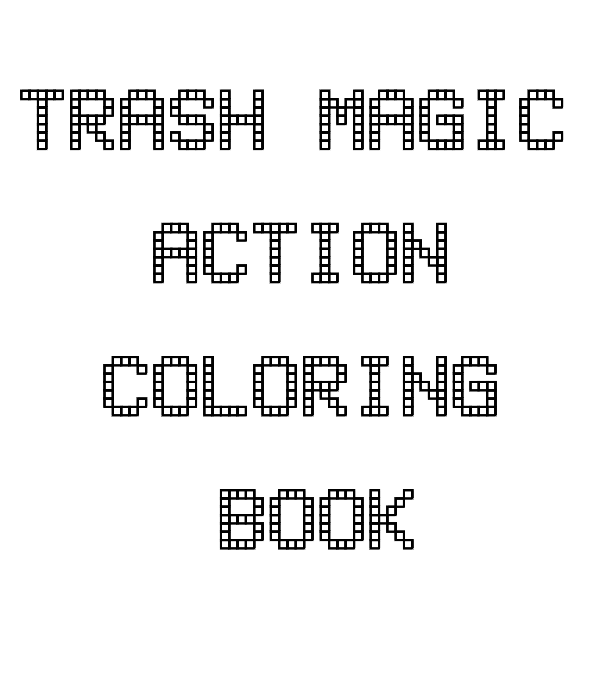
\includegraphics{cover.png}
%\end{figure}

\clearpage

\clearpage

\newpage
\thispagestyle{empty}
\mbox{}

\maketitle

%\tableofcontents

%\listoffigures 

%civilizations
%

\mainmatter

\chapter{Trash Magic}



We will build a world of both comfort and adventure from the waste streams of the old world.  We will use the trash we find everywhere to build all the things of a good life right where we are.  We will power this technology only with the sun, wind and water.  We will abolish all mining, oil, and gas by 2050.

Magic is the replication of the desire to replicate something.  If someone builds something out of trash which someone else wants to copy, and which will lead to still more people copying it, that's trash magic.  

Full trash magic is when we have trash magic technologies which taken together provide for all the things we need for a very good life.

To build this we will create Trash Factories.  A Trash Factory is a manufacturing hub which consumes waste from the local environment and converts it into products to directly provide to people in the local community.  Trash factories use only what is in their immediate physical environment for motive power.  This primarily means human power, direct solar heat, flowing water from rivers or tides, and wind.  It can be electrical, but can also be direct mechanical, as was common before universal electrification.  

Trash factories aim to close the loop of machine replication. This means we want the factories to have metal shops with all the basic tools of machine fabrication: milling machines, lathes, drill press, plastics welding and molding, welding and soldering, sheet metal working, etc.  With all these basic mechanical fabrication tools, we can in turn make more of these tools in that shop, using waste streams of metal found in our community.  

In order for trash factories to propagate, we will need very simple and clear instructions built into self-replicating media which describe how to replicate each part.  We also need a training corps who will go and recruit people to build trash factories and teach them how to do it.  Instructions should themselves be replicated as many times as possible, with new people recording their own videos on video sharing platforms, so that our media keeps improving.  

This book is a magic book, which will be self-described in the next chapter.  The fact that this book replicates means that as we add little bits and pieces of full trash magic, it will replicate as the book is copied and edited out in the wild.  

In addition to the machine shop, trash factories will be centered around textile fabrication again from waste.  We will use the machine shop to build machines for drawing plastic waste out into filaments, spinning it into thread, weaving it into cloth, and stitching it into clothes.  We will build machines for blending different materials into custom fibers for our own textiles which are based on what we can get our hands on. 

The textile part of the factory is our main initial product.  We need to have fiber arts experts and fashion designers involved at all stages of putting this together, so that we can build both practical and awesome looking stuff, custom designed for all body types.  Because we are supplying only our physically local community, all clothes are custom by default.  Our first priority in all clothing production is to provide survival gear to the most vulnerable people in our immediate physical community. From there we aim to create new fashions which blend practicality and comfort with post apocalyptic trash witch rainbowcore aesthetic.

For motive power we need the machine shop to also immediately be constructed around a standardized solar heat engine of some kind which can drive about 500-1000 watts, as well as a standard equivalent with wind and water.  This needs to have again a standardized system of shafts, pulleys and belts for power transfer to various machines as we add them as well as to electrical generators.  

For energy storage we need a standard water turbine and pump design which can be used to pump water uphill then run it downhill to get the energy back out.  We also need a battery solution we can make with safe waste streams.  We do not care about getting insanely high energy density or low weight.  Many ideas should be explored but we think the aluminum carbon cycle is perhaps the best choice, as we can get aluminum from beverage containers and carbon from locally produced charcoal.  Also, we need to create a reliable process for combining spent lithium ion cells and bringing them back to life.  

All the parts of the trash factory are intended to be things which can be either a purely trash-factory built thing or a off the shelf thing we can buy as we get started.  We cannot expect to build a fully closed loop trash factory immediately.  We instead aim to get something which creates value as fast as possible. 

Trash Camps are mutual aid centers in public spaces where we provide direct help to people in those spaces.  These camps are the retail distribution for the products we make in the trash factories.  Our aim with trash camps is to as quickly as possible have them provide some value to people in their infrastructure on site as well as a distribution point for a flow of free things to the most disenfranchised.

Trash academies are centers of learning for the community to learn about technology which is relevant to the trash magic system.  This includes both vocational training directly in how to operate the parts of the trash factory and more general education in all of the things we hope young people to know in the trash magic future.  What makes a trash academy different from an existing school is the lack of formal organizational structure but the much more clear intention of all the work done.  We might do this work in a public library, a university, a public park, on a huge raft made of trash, in a government lab or under a bridge. But wherever we do it we will do everything with the constant vision in mind that all our labors are in the direction of full trash magic.

Initially our trash academy education will have a few specific topics which we can immediately share in trash camps as a form of mutual aid because it can help people to survive right now.  This includes teaching people to make their own web pages, teaching them to make their own web-based applications, teaching people to build their own wireless networks, to build their own off-grid power.  We also have an open source Arduino development class.  If we build basic educational tools into the trash camps, and we have highly qualified technical instructors, we can mix teaching the most under-resourced students with helping the more privileged students whose families can then help us with resources.  

The trash academies will ultimately also serve as centers for research and development as we grow.  However, again, our initial focus is to provide value and to replicate first.  So initially we focus on the maximum educational benefit to the most disenfranchised, which is primarily technology education for getting direct control of their own social media platforms using the magic books(see next chapter).  Focusing on technology education allows us to 

\begin{figure}
	\centering
	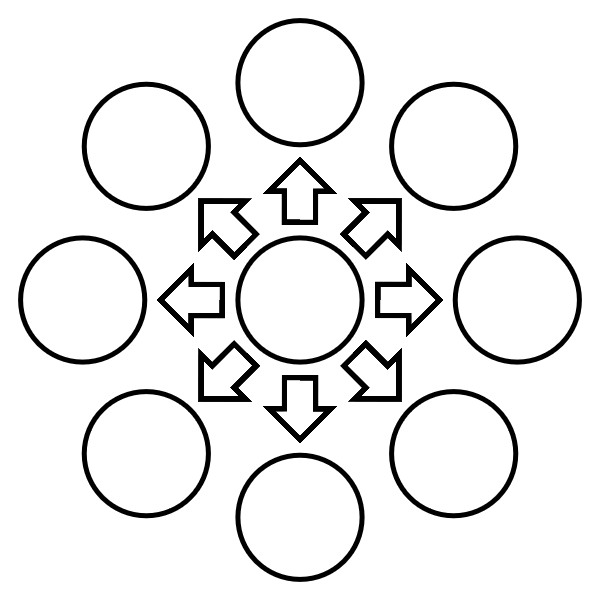
\includegraphics[width=4in]{imageserver/uploadimages/image12.png}
	\caption{Magic.}
\end{figure}

\begin{figure}
	\centering
	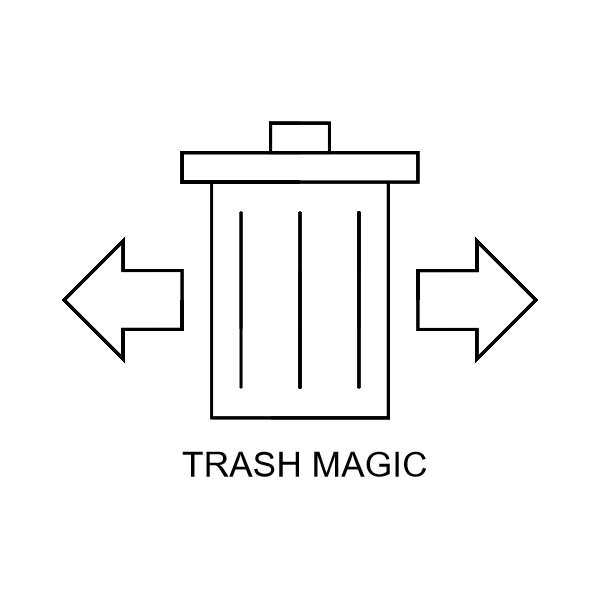
\includegraphics[width=4in]{imageserver/uploadimages/image13.png}
	\caption{Magic trash.}
\end{figure}

\begin{figure}
	\centering
	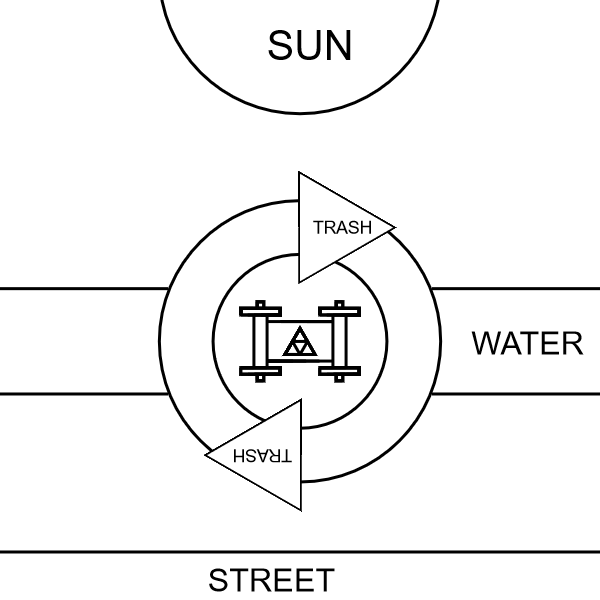
\includegraphics[width=4in]{imageserver/uploadimages/image14.png}
	\caption{Trash magic map.}
\end{figure}

\begin{figure}
	\centering
	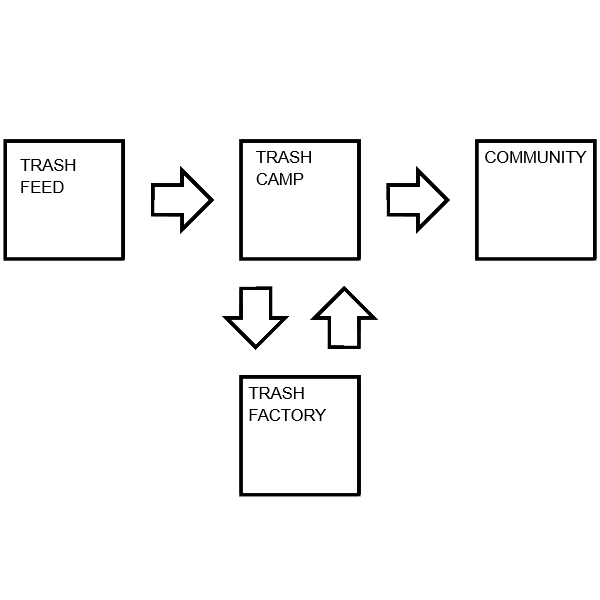
\includegraphics[width=4in]{imageserver/uploadimages/image15.png}
	\caption{Trash magic graph.}
\end{figure}



\chapter{Magic Book}
The magic book is a book which you co-create with other readers and writers.  It can replicate freely along the Geometron network, as described in the Book of Geometron.  This is not a specific book so much as a collection of methods of creating self-replicating books.  

The formats of the books are hand drawn and hand bound zines, bound 6x9 hard copy printed by print on demand Lulu press, printed letter size paper in three ring binders, and a web-based format which is how text is edited.  The web books have code in them which allows them to replicate freely from one Geometron server to another.  

As a keeper of any given version you will have received it from someone who can show you how to pass it along.  You can just pass along a book from one person to another and track it in the Street Network chapter. 

The electronic magic book can be part of an event, including a virtual one, where people message additions to a document to a human operator who edits the document in real time and shares it over a web server with everyone, who can then replicate it again, edit it again and so on.  This can be done on a Raspberry Pi, the cheap open source computer platform used for everything in the Geometron network. 

The Magic book can be used for many things. It can be used to co-create a story.  It can be used to create a shared book documenting a local community. It can be fiction or non-fiction.  It can be many hundreds or even thousands of pages, or just a single page with a short list of links.  It can be entirely images or just text.  What makes it magic is that it can always be replicated and edited by each new person we share it with.  As with trash magic, this fits our working definition of magic: the book replicates the desire to replicate the book.  

The Magic Book can also have oral formats, either from memory in person, over live stream, on a video sharing platform, or on an audio podcast.  Or it can be entirely performance art as we carry out the actions which are encoded in the book, just building and sharing geometry. 

\begin{figure}
	\centering
	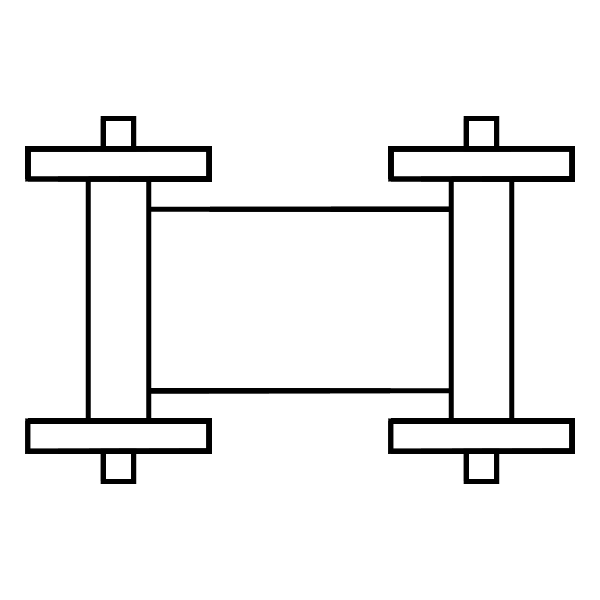
\includegraphics[width=4in]{imageserver/uploadimages/image16.png}
	\caption{Scroll.}
\end{figure}

\begin{figure}
	\centering
	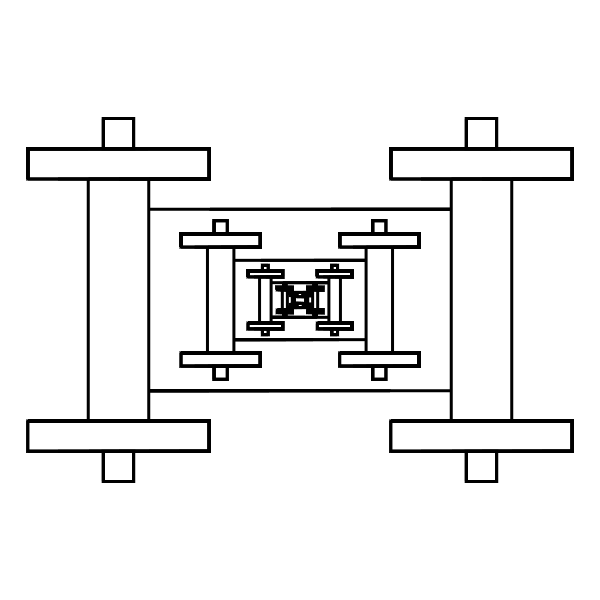
\includegraphics[width=4in]{imageserver/uploadimages/image17.png}
	\caption{Infinite scrolls.}
\end{figure}

\chapter{Street Network}

 \begin{figure}
	\centering
	
\includegraphics[width=4in]{imageserver/uploadimages/image3.png}
	\caption[streetmaps]
	{Draw maps for the region's streets, one for the major highway corridor, one for local major streets and one for the specific neighborhood.}
\end{figure}

 \begin{figure}
	\centering
	
\includegraphics[width=4in]{imageserver/uploadimages/image3.png}
	\caption[watermaps]
	{Draw maps for the region's water, one for the ocean and major shorelines of your watershed, one for major rivers or lakes and one for immediate drainage.}
\end{figure}

 \begin{figure}
	\centering
	
\includegraphics[width=4in]{imageserver/uploadimages/image3.png}
	\caption[people]
	{The path of this book: people.  Put your name, logo, symbols, signs, links, social media, contact as you see fit, then pass the book along to the next person.}
\end{figure}

 \begin{figure}
	\centering
	
\includegraphics[width=4in]{imageserver/uploadimages/image3.png}
	\caption[places]
	{Keep a record of the travels of this book.}
\end{figure}


\chapter{Trash Robot}

Trash robot is rainbow and googley eyes.   Trash robot is geometric constructions from cardboard with rainbow duct tape.   Trash robot is felt cutouts on black cotton flannel or sweat pants material.  Trash robot is post apocalyptic trash goblin energy.   Trash robot is chaos.  Trash robot is anarchist science. It's dirty kids in a school bus camper. It's a party by a dumpster.  It's running around in some steam tunnels.  It's weird art dropped in unexpected places. And of course it's robots built from trash.  When in doubt, add more rainbows, more googly eyes, more geometric constructions, and more trash and sticks and rocks.

Trash robot is an open brand.  All these aesthetic properties combined together can be very easy to recognize and replicate, but at the same time they are very clearly outside of any existing copyrights or trademarks.  By producing a large number of derivative works all in the public domain, we force the whole aesthetic to stay permanently in the public domain. If we build this into a powerful and valuable brand, that injects value into the public domain, which can be used to transmit all the rest of our technology also in the public domain. 

This whole structure is in analogy to how brands work in our existing economic system.  We aim to create a brand which stimulates free replication of free things in the same way a company uses their brand to sell their stuff.  This is not like the logos for an open source software project, which are generally property of a non-profit corporation.  Trash robot is not a logo. It is a general aesthetic, like vaporwave or goblincore, which are simply not owned by anyone.  If a big company wants to coopt it, let them.   As long as it stimulates replication of our system, we gain from it.  Attention will stimulate replication, so that's what we want.  
\chapter{Action Geometry}

Action Geometry. 



%\printindex

%https://www.sharelatex.com/learn/Glossaries

\end{document}